\section{Further consideration of machine vision aspects of the survey phase (J.~Kang)}
\label{sec:vision}

The purpose of this section is to discuss plant identification and image stitching, two necessary machine vision applications that would increase the chances of the survey mission successfully locating specimens of interest for retrieval. 

\subsection{Plant Identification}
Plant Identification is identifying plants with the survey drone using premade software. This was a low priority element of our CAPSTONE, but the research was important in case future groups wanted to implement it into their design. 

\subsection{Softwares and Methods}
\begin{itemize}
\item PlantId
\begin{itemize}
\item Free software 
\item Requires an upload of five plants weekly to maintain subscription
\item Seems to only work on image uploads and some plants may require multiple images of the same plant for proper identification
\item Would be difficult to implement into our system.
\end{itemize}
\item Convolutional Neural Networks
\begin{itemize}
\item This is basically deep learning for computer imaging. To a computer, an image is just a large matrix of RGB values, and it is possible to train a computer to recognize these RGB values and create a probability of what the image is about.
\item The process begins with neurons and weight. Each neuron can be thought of as a feature filter and uses small pixel sections of the entire image to determine what feature that pixel section represents.
\item Each pixel section uses its filter to output a number and these new numbers now can be used to determine higher level features, they now act as neurons going through a new filter. This can be visualized as a neural network. 
\item This process must be trained by using many different images. Each time the CNN is trained it alters the weights of its filter choices in order to improve its classification. This training process is what makes a CNN considered a deep learning algorithm. 
\item Further details of CNNs can be found in this link \url{https://adeshpande3.github.io/A-Beginner\%27s-Guide-To-Understanding-Convolutional-Neural-Networks/}
\end{itemize}
\item iNaturalist
\begin{itemize}
\item This software is similar to PlantId, but it is used for all animal life.
\item The identification does not come from code but from crowdsourcing done by experts in order to identify a specimen.
\item Images or Video taken from the survey drone can be uploaded to the iNaturalist website and await results from experts there.
\end{itemize}
\end{itemize}
\begin{figure}
\begin{center}
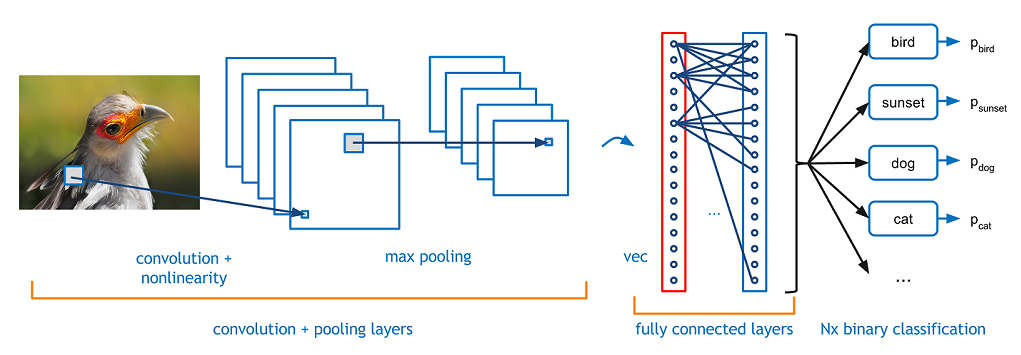
\includegraphics[width=\columnwidth]{figures/vision1.png}
\end{center}
\caption{Image taken from \url{https://adeshpande3.github.io/A-Beginner\%27s-Guide-To-Understanding-Convolutional-Neural-Networks/} to explain convolutional neural networks (CNNs).}
\end{figure}

\subsection{Image Stitching}
The vision for image stitching is to use images taken by the survey drone to recreate a map of the survey area. 


The following images and code were taken from \Matlab\ to provide an example on panoramic image stitching. In this folder contain two codes: \lstinline{ImageStitch.m}, my code (appendix~\ref{app:C2}), and \lstinline{FeatureBasedPanoramicImageStitching.m} (appendix~\ref{app:C1}), code taken from \Matlab. \lstinline{ImageStitch} is code I created in order to replicate \Matlab’s code for testing my own images taken from my room. After hours spent trying to fix it, there are still some problems that I cannot figure out. The problem seems to stem from the image format and pixel size, and I cannot figure out why the images are rotated \ang{90} when imported into \Matlab.

Figures~\ref{fig:vision1} and \ref{fig:vision2} show the result of running \Matlab’s code using their source images. It works extremely well and figuring out image formatting and more time with this code can mean creating image stitched maps of our own for the survey mission.
  
\begin{figure}
\begin{center}
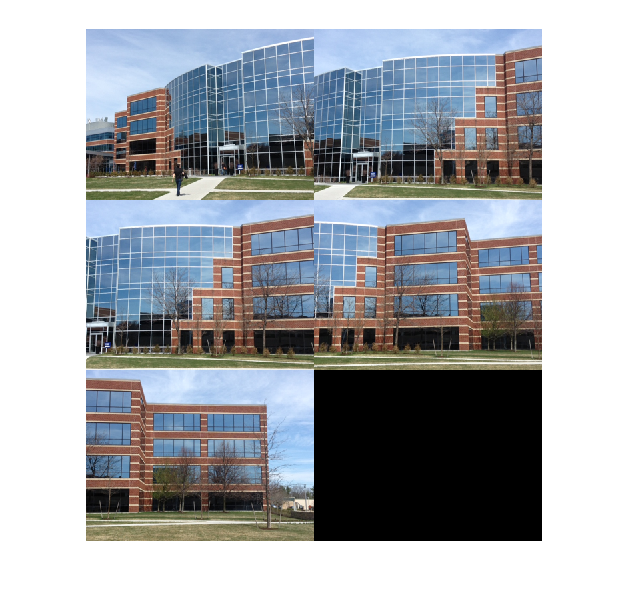
\includegraphics[width=0.8\columnwidth]{figures/vision2.png}
\end{center}
\caption{Five Images of a Building}
\label{fig:vision1}
\end{figure}
  
\begin{figure}
\begin{center}
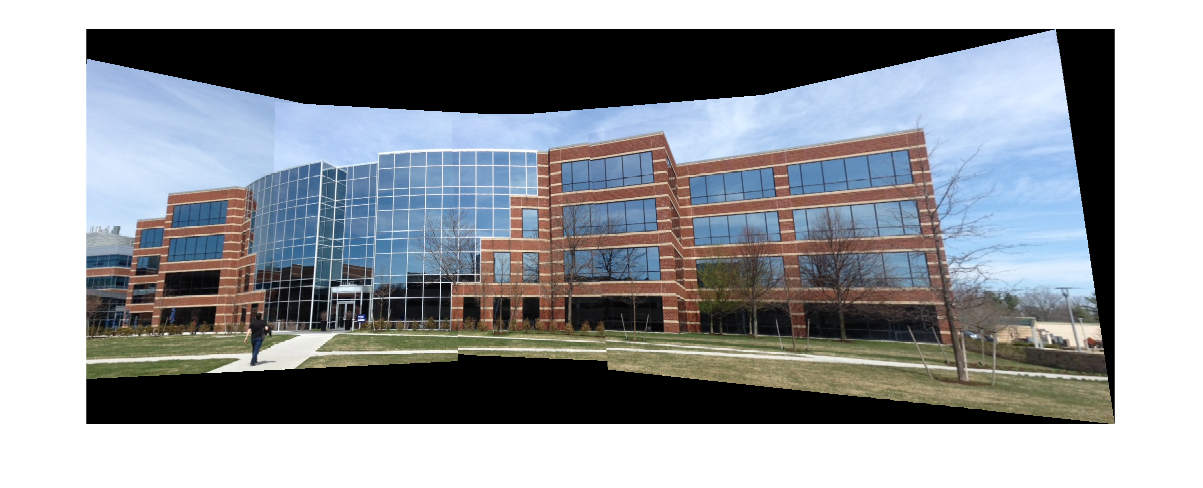
\includegraphics[width=\columnwidth]{figures/vision3.png}
\end{center}
\caption{The Images Connected through Feature Based Panoramic Image Stitching}
\label{fig:vision2}
\end{figure}